\chapter{MARCO TEÓRICO}
	\section{Geofísica y Geoeléctrica}
		\subsection{Definición de Geofísica}
			
			En términos generales la geofísica es la aplicación de los principios físicos de la materia en el estudio del planeta Tierra, o cual quier otro cuerpo celeste, desde el campo magnético, pasando por los fenómenos atmosféricos al medio solido del subsuelo, hasta las profundidades del núcleo interno planetario, ya sea que se aproveche una fuente natural como la propagación de ondas elásticas generadas por sismo, ó bien, la inducción de campo electromagnético de fuente controlada \citep{parasnis2012, reynolds2011, lay1995}.   
		
			El  nacimiento de la geofísica es relativamente reciente, la primera prospección geoeléctrica data de 1830 realizados por \cite{fox1830} en Cornwal, Reino Unido, donde aplico técnicas de Self-Potential en exploración de mineralización de sulfuro en vetas, la medición del potencial natural resulto altamente efectiva para la prospección de este tipo de mineralizaciones ya que su anomalía se caracterizaba por presentar una respuesta muy marcada con respecto al medio \citep{reynolds2011, revil2013}.
			
		\subsection{Resistividad de la Tierra}
				
			De manera general la materia presenta propiedades físicas definidas a partir de los elementos que la integran, en primer orden la configuración atómica establece las propiedades físicas, estas se definen a partir de la estructura de electrones, protones y neutrones que presentan los átomos; a su vez, las moléculas pueden estar conformadas por una clase especifica de átomos (moléculas homonucleares) o por conjuntos de diferentes tipos (compuestos), cuya conformación depende de factores físico-químicos \citep{tiab2024}.
			
			La configuración molecular inorgánica presente en la materia, definirá el tipo de estructura cristalina (mineral) que formarán, y por consiguiente esta provista de propiedades físicas definidas en base a su composición y estructura; esta configuración cristalina es la que encontramos en el medio geológico conformando los minerales que componen la estructura mineral de una unidad geológica (ver figura \ref{fig:eo}) \citep{gandhi2016, tiab2024}.\\
			
			\begin{figure}[h!]
				\centering
				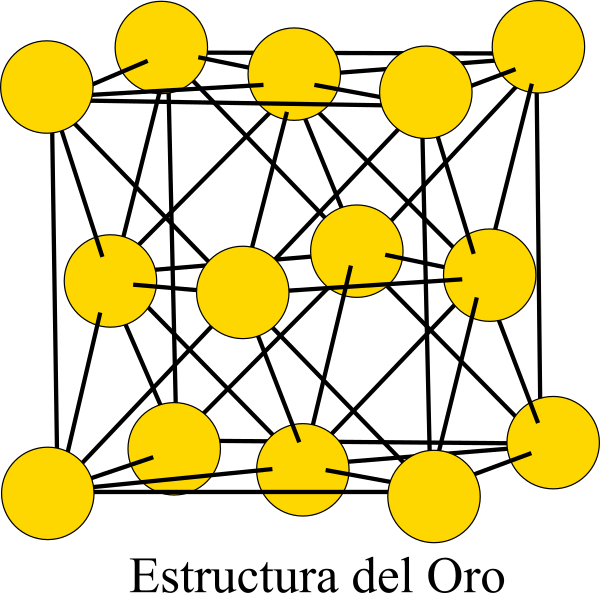
\includegraphics[width=5cm]{Imagenes/estructura-oro}
				\caption[Estructura atómica del oro]{Esquema de la estructura atómica de oro que conforma la cristalización octahedral, modificado de \citet{sorrell1973}}.
				\label{fig:eo}
			\end{figure}
			
			Los métodos Geoeléctricos se clasifican en dos grupos, métodos pasivos y de inducción, los primeros corresponden a aquellos en los que se mide el potencial eléctrico natural, usualmente medido en mili volts, en donde se requiere de electrodos no polarizables para tener medidas lo más claras posibles; mientras que los métodos de inducción emplean un arreglo de electrodos, o inductores de campo electromagnéticos, mediante los cuales se induce un campo eléctrico al subsuelo, calculando la diferencia de potencia eléctrica en el medio, o bien, el decaimiento de la polarización inducida \citep{revil2013, reynolds2011, igboama2023}.
			
			Los métodos de inducción, Sondeo Eléctrico Verticales (VES, por sus siglas en inglés), Tomografía de Resistividad Eléctrica (ERT, por sus siglas en inglés), Polarización Inducida (IP, por sus siglas en inglés), presentan una gran ventaja ya que no dependen del medio para poder realizar una lectura, ademas de poder realizarlos en cualquier momento, manteniendo el equipo en condiciones de operación, y pode diseñar arreglos de adquisición que nos permitan tener un muestreo tan amplio o limitado como sea conveniente, solo limitados por el alcance y potencia de los equipos empleados. Por otro lado su interpretación presenta un alta ambigüedad, solo acotado por la cantidad de referencias que puedan cruzarse para robustecer el modelo geológico y de inversión, y así poder llegar a una interpretación satisfactoria \citep{reynolds2011, igboama2023}.
			
			El método de prospección geoeléctrica, en especifico el SEV y la TRE, consiste en determinar la distribución de resistividades del subsuelo, de manera que se pueda establecer una correlación entre la resistividad y un modelo ajustado a la realidad geológica-estructural, geotécnica o geohidrológica del objeto de estudio.
	
		\subsection{Sondeo Eléctrico Vertical}
			
			Los SEV corresponden al método de mas rápida ejecución y económicamente mas accesible, por lo que es ampliamente empleado para solucionar problemas de ingeniería, minería, geotecnia, monitoreo e impacto ambiental y abastecimiento de Aguas potable; siendo de gran utilidad en la exploración de hidrogelogica ya que la respuesta resistiva de un medio saturado permite establecer diferencias concisas y discriminar entre agua dulce, salada, rocas fracturadas, arcillas , arenas, conglomerados, etc.
			
			La resistividad es medida mediante la inyección de una corriente en el subsuelo y mientras que se monitorea y captura la diferencia de potencial eléctrico en la superficie, esta lectura corresponde al valor de la contribución resistiva de todas las capas por donde fluye la corriente.
			
			La inyección de corriente y medición del potencial se realiza a través de un arreglo de dos pares de electrodos, $A, B (C_{1}, C_{2})$ y $M, N (P_{1}, P_{2}) $ respectivamente, siendo el electrodo $A (C_{1})$ el polo positivo y $B (C_{2})$ el polo negativo de inyección, mientras que el electrodo $M (P_{1})$ corresponde al polo positivo y $N (P_{2})$ al polo negativo de los electrodos de potencial.\\
			 
			\begin{figure}[h!]
				\centering
				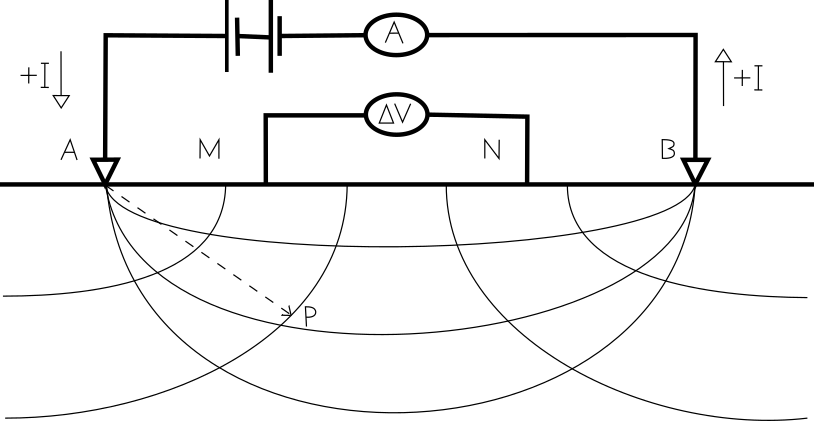
\includegraphics[width=9cm]{Imagenes/ArregloElectrodos}
				\caption[Configuración general de electrodos]{Configuración general de arreglo de electrodos, modificado de \citet{reynolds2011}}.
				\label{fig:AE}
			\end{figure}
			La resistividad del subsuelo se calcula a partir de la ley de Ohm, considerando el caso general en donde el medios es homogéneo y el arreglo de electrodos presenta una distribución convencional, donde se establece una relación directamente proporcional entre la la resistencia $R$ ,medida en Ohm ($\Omega$), y el cociente entre la diferencia de potencial $\Delta V$ y la corriente inducida $I$, para un valor puntual \citep{igboama2023}.
			
			\begin{equation}
				R = \frac{\Delta V}{I}
			\end{equation}
			   
			Sabiendo que se puede calcular $R$ para una sección con longitud $L$ y un área $A$, transversal del material, conociendo la resistividad ($\rho$) del material \citep{igboama2023, lowrie2020}, podemos reescribir la ecuación como: 
			
			\begin{equation}
				R = \rho \frac{L}{A}  \rightarrow  	\rho  = R \frac{A}{L} \rightarrow \rho  = R \cdot k
			\end{equation}
			
			Donde la resistividad ($\rho$) es una constante de proporcionalidad del medio y $k$ es el factor geométrico de distribución del flujo de corriente en términos de la del arreglo  de los electrodos de inducción y potencial (distancias entre los electrodos A-M-N-B ) \citep{igboama2023, lowrie2020}.
			
			\begin{equation}
				k = 2\pi \left(  \dfrac{1}{AM} - \dfrac{1}{AN} - \dfrac{1}{BM} + \dfrac{1}{BN} \right) 
			\end{equation}
			
			Tenemos que la resistividad aparente ($\rho _{A}$) de una sección del subsuelo, corresponde a la contribución resistiva de las unidades geológicas en esa sección, en términos de las distancias entre electrodos, la diferencia de potencial y el flujo de corriente en el medio \citep{igboama2023, lowrie2020}, esta dado por la siguiente ecuación:
			
			\begin{equation}
				\rho_{A} = \frac{\Delta U}{I} \cdot k %\rho_{A} = 2\pi \cdot \frac{\Delta U}{I} \cdot k
			\end{equation}
			
			\subsubsection{Arreglo de Electrodos y Factor Geométrico}
			
				Cada arreglo presenta ventas, desventajas, rango de sensibilidad y espacio de ejecución, debido a estas características y se tiene que evaluar e identificar que arreglo cumple con las condiciones adecuadas para ser ejecutado, considerando el espacio disponible en el sitio de estudio, el nivel de ruido (motores, conexiones a tierra mal aterrizadas, antenas, postes metálicos, arboles), la profundidad de objeto de prospección y la resolución vertical alcanzable (ver figura \ref{fig:Contri}).
				
					\begin{figure}[h!]
						\centering
						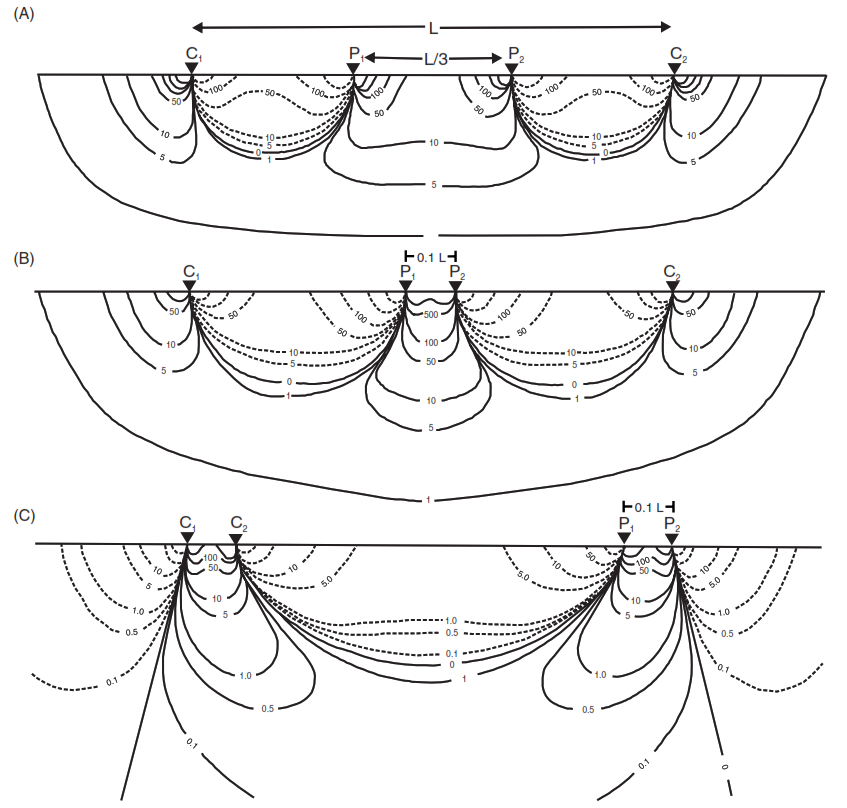
\includegraphics[width=12cm]{Imagenes/5}
						\caption[Esquema de la contribución de la respuesta eléctrica]{Esquema de la contribución de la respuesta de resistividad eléctrica, modificado de \citet{reynolds2011}}.
						\label{fig:Contri}
					\end{figure}				
				
				Como se observa en la sección anterior, la resistividad se determina empleando una configuración de los electrodos durante una medición, las distintas configuraciones de electrodos se encuentran ampliamente documentadas, cada una presenta un factor geométrico distinto \citep{igboama2023, lowrie2020}, los principales arreglos geoeléctricos son:
				
				\begin{description}
					\item[Wenner ]  
							\begin{equation}
								\rho_{A} = 2\pi \cdot R \cdot a
							\end{equation}
							
							\begin{figure}[h!]
								\centering
								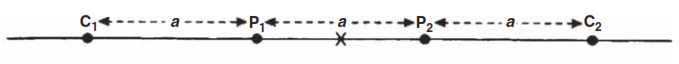
\includegraphics[width=9cm]{Imagenes/1}
								\caption[Esquema del arreglo Wenner]{Esquema del arreglo Wenner, modificado de \citet{reynolds2011}}.
								\label{fig:AW}
							\end{figure}
							
					\item[Schlumberger ] 
					
						\begin{equation}
							\rho_{A} = \frac{\pi a^{2}}{b} \left[ 1 - \frac{b^{2}}{4 a^{2}} \right] \cdot R, \quad a \geq 5b
						\end{equation}

							\begin{figure}[h!]
								\centering
								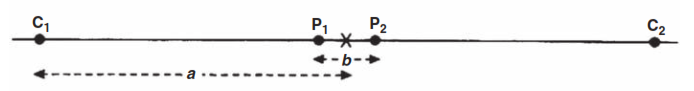
\includegraphics[width=9cm]{Imagenes/2}
								\caption[Esquema del arreglo Schlumberger]{Esquema del arreglo Schlumberger, modificado de \citet{reynolds2011}}.
								\label{fig:AS}
							\end{figure}
					
					\item[Dipolo-dipolo]  
					
							\begin{equation}
								\rho_{A} = \pi n(n+1)(n+2)a \cdot R
							\end{equation}
					
							\begin{figure}[h!]
								\centering
								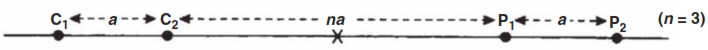
\includegraphics[width=9cm]{Imagenes/3}
								\caption[Esquema del arreglo Dipolo-dipolo]{Esquema del arreglo Dipolo-dipolo, modificado de \citet{reynolds2011}}.
								\label{fig:ADD}
							\end{figure}
				\end{description}
	
	\section{Adquisición de Datos Geofísicos}
	
	Previo al trabajo de adquisición se realiza un análisis de entorno, en el cual se verifica la viabilidad del arreglo dadas las condiciones del sitio, considerando lo siguiente: espacio disponible en el sitio de estudio, profundidad de exploración, nivel de ruido eléctrico, interferencias con la estabilidad del potencial natural del subsuelo, profundidad del objeto de exploración y dimensiones aproximadas del mismo.
	
		\subsection{Intervalo de Muestreo en SEV}
			
			El intervalo de muestreo empleado durante la adquisición de un SEV es un parámetro crítico que influye en la calidad y precisión de los datos geofísicos adquiridos, ya que esta estrechamente relacionado con la resolución vertical que deseamos de acuerdo al objeto de estudio. Durante la planeación es necesario considerar distintas condiciones, como son:
			
			\begin{itemize}
				\item Los espesores de cada unidad.
				\item La distribución de las distintas unidades.
				\item Profundidad de investigación
				\item Ruido en la señal.
			\end{itemize}
			
			Para establecer un intervalo de muestreo apropiado, se deben considerar el Teorema de Muestreo de Nyquist y El teorema de Shannon-Hartley (teorema de codificación de canal ruidoso), al igual que la geometría del arreglo geoeléctrico empleado.
			
			El Teorema de Muestreo de Nyquist, el cual, es un principio fundamental en el procesamiento de señales analógicas y digitales, establece las condiciones mínimas necesarias para la reconstrucción una señal analógica a partir de muestras discretas \citep{alvarado2010}.
			
			Nyquist nos garantiza las condiciones necesarias y suficientes para llevar a cabo una adquisición exitosa de muestreo de una señal, llámese distribución de resistividad en un medio heterogéneo y discontinuo \citep{alvarado2010}, considerando siempre los espesores como inferidos a partir de muestreo directo.
			
			\begin{equation}
				f_{s} \geq 2 \cdot f_{max}
			\end{equation}
			
			Donde la frecuencia de muestreo $f_{s}$ es por lo menos dos veces mayor a la frecuencia máxima $f_{max}$ conocida, cuando el teorema no se cumple se genera una distorsión en la señal, sumando las frecuencias altas incompletas a la señal natural de baja frecuencia, generando ruido, y problemas de interpretación, se conoce como aliasing \citep{alvarado2010}. 
			
			Considerando el medio geológico como una región con presencia constante de ruido eléctrico de fuentes tanto naturales como humanas, es imprescindible considerar el teorema de Shannon-Hartley aplicando apilamiento de muestreo como método de reducción de la relación ruido señal, durante la adquisición de datos; esto quiere decir calcular el promedio de muestreos continuos en un intervalo definido de aperturas entre electrodos.
			
			%% agregar ecuacion de shanon y desgrlosar sus elementos e interpretacion
				
			\subsubsection{Factores que Determinan el Intervalo de Muestreo}
		
				En el contexto de la adquisición de datos mediante SEV, el intervalo de muestreo es equivalente al espaciado entre puntos donde se realizan mediciones de resistividad del subsuelo. Este intervalo de muestreo debe ser lo mas pequeño posible, de modo que permita obtener muestras de resistividad \citep{telford1990}, esta relación se define de la siguiente manera:
				
				\begin{equation}
					f_{s}= \frac{1}{\Delta x}
				\end{equation}
				
				Donde el intervalo de muestreo $\Delta x$ debe ser menor a la mitad de la longitud de onda ($\lambda_{min}$, espesor) asociado al objetivo de exploración.
				
				\begin{equation}
					\Delta x \leq \frac{\lambda_{min} }{2}
				\end{equation}
				
				
			
		\subsection{Proceso de Adquisición In Situ}
			La adquisición de datos se realiza mediante la lectura directa en campo, tomando una primera lectura del potencial natural por medio de los electrodos M y N, se continua con la lectura al inducir corriente continua empleando un resistivímetro mediante los electrodos de corriente A ($C_{1}$) y B ($C_{2}$), mientras se realiza la lectura de potencia en los electrodos M ($P_{1}$) y N ($P_{2}$), la lectura se realiza en intervalos regulares en instantes de inyección de corriente \citep{telford1990}.
			
			Durante la toma de datos es importante considerar los modelos previos realizados durante el análisis preliminar, ya que las resistividades esperadas para las unidades, permiten tener control en la dispersión de datos, identificando tomas erróneas y corrigiendo al momento con una nueva lectura \citep{telford1990}.
	
	\section{Machine Learning en la Geofísica}  
	
	La aplicación de ML en la geofísica es utilizado en exploración sísmica, abarcando los procesos de adquisición, mejorando los tiempos de procesamiento, clasificación e interpretación, ya que es en este método donde se cuenta con la mayor cantidad de datos para entrenamiento \citep{wrona2018}; en menor medida se implementan técnicas de ML en la exploración y prospección geoeléctrica, hay algunos ejemplos destacables como son \cite{liu2020, el2001, li2024}, sin embargo no es un estándar en la metodología, pese a las ventajas que puede tener su aplicación, como se pretende demostrar en este estudio.
		
	El machine learning se integra por conjunto de técnicas que utilizan algoritmos con los cuales permite a un sistema aprender y generar predicciones, para lo que requiere un conjunto de datos para poder realizar el entrenamiento.
	
	Podemos clasificar los algoritmos de ML por el tipo de entrenamiento que ejecutan, correspondiendo a aprendizaje supervisado, no supervisado y por refuerzo, y por la relación que establecen con los parámetros del conjunto de datos de entrenamiento, es decir, modelos paramétricos y no paramétricos \citep{li2024}. 
	
	De los modelos no paramétricos destacan por su adaptabilidad a la estructura subyacente de los datos, por lo que pueden realizar aprendizaje de relaciones complejas entre datos, así como ausentes de linealidad, teniendo un costo en volumen de datos, requiriendo un número mayor para su entrenamiento, destacan los siguientes algoritmos de ML.
	
	\begin{itemize}
		\item Random Forests
		\item Support Vector Machines 
		\item Gradient Boosting Regression
	\end{itemize}
	
	Dada la naturaleza de los datos de SEV's, heterogéneos, discontinuos y no lineales, es conveniente abordar su analistas desde un enfoque no paramétrico, teniendo esto en cuanta, los métodos empleados destaca siendo eficaz en la tarea de clasificación y regresión, teniendo algunos beneficios como son la reducción del sobre ajuste, interpretación de variables, resistencia al aliasing.
	
	\section{Random Forests} 
	
		Random Forests es una técnica propuesta por \citet{breiman2001}, la cual emplea múltiples arboles de decisión independientes entre si, donde cada árbol realiza una votación de clases, seleccionando la más popular de la entrada de cada árbol realizando una combinación de salida, permitiendo realizar una clasificación de características complejas o realizar regresiones de datos complejos multivariables \citep{breiman2001, lan2020}.
		
		La herramienta de Random Forests, de acuerdo con \citet{breiman2001} emplea tres elementos clave en el proceso de entrenamiento, bagging, selección aleatoria de características y agregación por votación, resultando en la combinación del los resultados en una predicción o clasificación robusta y ajustada \citep{lan2020}.
		
		\subsection{Bootstrap aggregating}
			
			
			Esta característica de Random Forest genera una colección de \textit{M} árboles de decisión no correlacionados, cada uno de ellos se entrena utilizando muestras aleatorias del conjunto de datos originales, identificados como datos de entrenamiento \textit{D}, este proceso se conoce como bootstrap aggregating \citep{breiman2001}.
			
			Deacuerdo con \citet{breiman2001}, Random Forests es un conjunto de clasificadores $H(x,\theta_{k})$, $x$ es un vector de entrada y $\theta_{k}$ corresponden a vectores aleatorios independientes generados a partir de los datos de entrenamiento $D$, con árboles $k$ (donde $k = 1, 2, ..., M$), esta aleatoriedad puede generar datos replicados en $\Theta_k$, mientras que otros arboles pueden estar faltantes. La dimensión $\Theta_k$ es aproximadamente el 80\% del tamaño de $D$.
			
		\subsection{Selección Aleatoria de Características}
			
			Al construir cada árbol, en cada nodo, en lugar de considerar todas las características para encontrar la mejor división, se selecciona aleatoriamente un subconjunto de $K$ características
			
			En cada nodo de los subconjuntos de entrenamiento se selecciona una características por votación de popularidad, dejando crecer cada árbol sin realizar poda hasta completar los criterios de finalización, es decir un numero de instancias preestablecido\citep{breiman2001}.
			
		\subsection{Predicción por Agregación}
		
			 La clasificación para una entrada $x$ se basa en las predicciones individuales de los árboles para cada clase $h_{k}(x)$, se realiza un conteo de cada clase, producto de la predicción de cada árbol, sumando las salidas $I(h_{k}(x)=c)$, y finalmente se selecciona clase con mayor numero de predicciones, obteniendo la predicción de clasificación $H(x)$,donde $x$ es una función indicadora que vale 1 si $h_{k}(x)=c$, y $0$ en caso contrario \citep{breiman2001}.
			 
			 \begin{equation}
			 	H(x) = \text{argmax}_c \sum_{k=1}^K I(h_k(x) = c)
			 \end{equation}


			El proceso de la regresión se obtiene a partir de la media aritmética de cada predicción individual, donde cada árbol produce un valor numérico $h_{k}(x)$ correspondiente a cada $x$, al corresponder con promedio de las predicciones se le otorga mas estabilidad cuando tenemos un numero elevado de arboles  y un conjunto de datos grande, entendiéndolo como un modelo central que incorpora información de cada árbol \citep{breiman2001}. 
			
			\begin{equation}
					H(x) = \frac{1}{K} \sum_{k=1}^K h_k(x)	
			\end{equation}

		\subsection{Varianza y Overfitting}
		
			Algo notable en el algoritmo Random Forest es su capacidad para reducir la varianza sin que esto afecte significativamente el sesgo, lo que ayuda a evitar el overfitting (sobre ajuste), ya que el bagging, ejecutado durante el proceso de bootstrap, reduce la varianza al promediar las predicciones de múltiples modelos entrenados en diferentes árboles. La selección aleatoria de características descorrelaciona aún más los árboles, lo que contribuye a la reducción de la varianza \citep{breiman2001,veirana2021}.
			
			La varianza de un Random Forest puede expresarse aproximadamente como:
			
				\begin{equation}
					Var ( JM_{RF} ) = \rho(x)\sigma^2 + \frac{1 - \rho(x)}{M}\sigma^2
				\end{equation} 
				
			Donde $\sigma^2$ es la varianza promedio de cada árbol y $\rho(x)$ es la correlación promedio entre las predicciones de cualquier par de árboles $k$. A medida que el número de árboles $M$ aumenta, el segundo termino tiende a cero, acercando la varianza a $\rho(x)\sigma^2$ \citep{breiman2001,veirana2021}.
			
		\subsection{Bias-Varianza Tradeoff}
		
		El objetivo en el aprendizaje automático es encontrar un modelo que minimice el error de prueba esperado ($E[E_{TEST}]$)\citep{breiman2001}, el cual puede descomponerse en sesgo al cuadrado ($Bias^2$), varianza ($Var$) y ruido ($Noise$): $$E[E_{TEST}] = Bias^2 + Var + Noise \quad$$
		
		Con el método Random Forest se busca un equilibrio entre sesgo y varianza, considerando que los árboles individuales por lo general tienen un bajo sesgo y alta varianza, siendo equilibrado por el proceso bootstrap al reducir la varianza del ensamble, resultando en un mejor rendimiento general en datos no vistos\citep{breiman2001}.
		
		
	\section{Support Vector Machines} 
	
	Este algoritmo de aprendizaje supervisado tiene como objetivo encontrar el hiperplano que mejor separa las clases en el espacio de características, maximizando la distancia entre este y los puntos más cercanos de cada clase, conocidos como vectores de soporte. En casos donde los datos no son linealmente separables, permite ciertas violaciones del margen mediante un parámetro de penalización que controla el equilibrio entre precisión y generalización, además, mediante el uso de funciones kernel, es posible proyectar los datos a espacios de mayor dimensión para lograr una separación lineal que no sería posible en el espacio original\citep{james2013, veirana2021}.
	
	En problemas de regresión se emplea la variante Support Vector Regression (SVR). En este caso, el modelo busca una función que se mantenga dentro de un margen de tolerancia $\epsilon$ respecto a los valores reales, permitiendo cierto grado de error controlado por variables de holgura\citep{james2013}.
	
	Tanto en clasificación como en regresión, SVM es una técnica robusta, especialmente útil en espacios de alta dimensión, aunque su desempeño depende de una adecuada elección de hiperparámetros y de kernel.
	
	
	\subsection{Hiperplano Separador}
	
	En la clasificación binaria más simple, cuando los datos son linealmente separables, el objetivo es encontrar un hiperplano que divida claramente las dos clases. En un espacio de $p$ dimensiones, dicho hiperplano se define por la ecuación \citep{james2013}:
	\[
	w^T x + b = 0
	\]
	donde:
	\begin{itemize}
		\item $w$ es un vector de pesos que determina la orientación del hiperplano,
		\item $x$ es el vector de características de una instancia,
		\item $b$ es un escalar que define la posición del hiperplano (sesgo).
	\end{itemize}
	Un hiperplano separador cumple que $w^T x + b > 0$ para una clase y $w^T x + b < 0$ para la otra.
	
	\subsection{Clasificador de Margen Máximo}
	
	El clasificador de margen máximo busca el hiperplano que maximiza la distancia (margen) entre las observaciones más cercanas de cada clase y el propio hiperplano \citep{james2013}. Estas observaciones se denominan \textit{vectores de soporte}.
	
	El problema de optimización se formula como:
	\[
	\underset{w, b}{\text{minimizar}} \quad \frac{1}{2} \|w\|^2 \quad \text{sujeto a} \quad y_i(w^T x_i + b) \geq 1, \quad i = 1, ..., n
	\]
	donde $y_i \in \{-1, 1\}$ representa las clases. Esta formulación garantiza la separación de clases con el mayor margen posible.
	
	\subsection{Clasificador de Margen Suave (Soft Margin)}
	
	Cuando los datos no son perfectamente separables, se introducen variables de holgura $\xi_i \geq 0$ para permitir ciertas violaciones del margen:
	\[
	\underset{w, b, \xi}{\text{minimizar}} \quad \frac{1}{2} \|w\|^2 + C \sum_{i=1}^{n} \xi_i \quad \text{sujeto a} \quad y_i(w^T x_i + b) \geq 1 - \xi_i
	\]
	Aquí, $C > 0$ es un hiperparámetro que controla el compromiso entre la maximización del margen y la penalización por errores de clasificación \citep{james2013, veirana2021}.
	
	\subsection{Método del Kernel}
	
	Para datos no linealmente separables, SVM emplea el \textit{truco del kernel}, que permite proyectar los datos a un espacio de mayor dimensión donde sí pueden ser separados linealmente, sin necesidad de calcular dicha proyección explícitamente \citep{james2013, veirana2021}.
	
	Funciones kernel comunes:
	\begin{itemize}
		\item \textbf{Lineal}: $K(x_i, x_j) = x_i^T x_j$
		\item \textbf{Polinomial}: $K(x_i, x_j) = (x_i^T x_j + r)^d$
		\item \textbf{RBF (Gaussiano)}: $K(x_i, x_j) = \exp(-\gamma \|x_i - x_j\|^2)$
		\item \textbf{Sigmoidal}: $K(x_i, x_j) = \tanh(\alpha x_i^T x_j + c)$
	\end{itemize}
	
	El problema de optimización dual con kernel se escribe como:
	\[
	\underset{\alpha}{\text{maximizar}} \quad \sum_{i=1}^{n} \alpha_i - \frac{1}{2} \sum_{i,j=1}^{n} \alpha_i \alpha_j y_i y_j K(x_i, x_j)
	\]
	\[
	\text{sujeto a} \quad \sum_{i=1}^{n} \alpha_i y_i = 0, \quad 0 \leq \alpha_i \leq C
	\]
	La función de decisión para una nueva instancia $x$ es:
	\[
	f(x) = \text{sgn} \left( \sum_{i \in SV} \alpha_i y_i K(x, x_i) + b \right)
	\]
	
	\subsection{Regresión por Vectores de Soporte (SVR)}
	
	SVM también puede aplicarse a regresión mediante SVR, cuyo objetivo es encontrar una función $f(x)$ que tenga una desviación máxima de $\epsilon$ respecto a los valores verdaderos, penalizando sólo los errores mayores \citep{james2013, veirana2021}.
	
	El problema se plantea como:
	\[
	\underset{w, b, \xi, \xi^*}{\text{minimizar}} \quad \frac{1}{2} \|w\|^2 + C \sum_{i=1}^{n} (\xi_i + \xi_i^*)
	\]
	\[
	\text{sujeto a} \quad 
	\begin{cases}
		y_i - (w^T x_i + b) \leq \epsilon + \xi_i \\
		(w^T x_i + b) - y_i \leq \epsilon + \xi_i^* \\
		\xi_i, \xi_i^* \geq 0
	\end{cases}
	\]
	
	Donde $\epsilon$ define una región sin penalización y $C$ regula el compromiso entre la planitud del modelo y la tolerancia a errores.

	
	
\section{Gradient Boosting Regression}

Gradient Boosting Regression es un método de aprendizaje ensamblado que construye modelos predictivos de manera secuencial. A diferencia de técnicas como Bagging y Random Forest, donde los árboles de decisión se construyen de forma independiente y se combinan al final, en Gradient Boosting cada nuevo árbol se entrena específicamente para corregir los errores cometidos por la suma de árboles anteriores. Esto permite una mejora progresiva en el desempeño del modelo a lo largo de múltiples iteraciones \citep{hastie2009, friedman2001}.

\subsection{Naturaleza Secuencial}

El modelo se construye de manera iterativa. Se inicia con una predicción base (por ejemplo, el promedio de las salidas) y, en cada iteración, se ajusta un nuevo árbol de decisión sobre los errores cometidos por la suma de modelos anteriores. El resultado es un modelo compuesto por muchos árboles débiles, cuya combinación forma un modelo fuerte.

\subsection{Minimización de la Función de Pérdida}

En cada iteración, el algoritmo intenta minimizar una función de pérdida $L(y_i, \hat{f}(x_i))$, que cuantifica la discrepancia entre los valores reales $y_i$ y las predicciones actuales $\hat{f}(x_i)$. La elección de la función de pérdida depende del tipo de problema (por ejemplo, el error cuadrático medio para regresión) \citep{james2013}.

\subsection{Ajuste a los Residuales}

El nuevo árbol se entrena sobre los \textit{pseudo-residuales}, definidos como el gradiente negativo de la función de pérdida con respecto a las predicciones actuales. En el caso de regresión con error cuadrático, estos pseudo-residuales coinciden con los residuales clásicos:
\[
r_i^{(b)} = y_i - \hat{f}^{(b-1)}(x_i)
\]
Esto permite que cada nuevo árbol aprenda los patrones de error que el modelo anterior no pudo capturar.

\subsection{Shrinkage (Tasa de Aprendizaje)}

Para evitar que cada nuevo árbol domine demasiado el modelo, se introduce un parámetro de \textit{shrinkage} o \textit{tasa de aprendizaje}, denotado como $\lambda \in (0,1)$ \citep{james2013, veirana2021}. Este factor escala la contribución de cada árbol:
\[
\hat{f}^{(b)}(x) = \hat{f}^{(b-1)}(x) + \lambda \cdot f_b(x)
\]
Valores pequeños de $\lambda$ (como 0.01 o 0.001) ralentizan el aprendizaje, lo cual puede mejorar la generalización del modelo.

\subsection{Regularización}

Además del parámetro $\lambda$, se pueden emplear otras técnicas de regularización, como la profundidad máxima de los árboles ($d$), el número mínimo de muestras por hoja, o la fracción de datos usados en cada iteración (submuestreo) \citep{james2013}. Estas estrategias ayudan a reducir la varianza del modelo y mitigar el riesgo de sobreajuste.

\subsubsection{Algoritmo de Gradient Boosting para Regresión}

Antes de implementar este algoritmo es importante entender su dinámica iterativa y cómo se construyen las predicciones dentro del algoritmo, en donde optimiza una función de pérdida específica de manera directa mediante técnicas de gradiente, agregando modelos débiles (árboles de decisión) que corrigen los errores residuales del conjunto de modelos anteriores. El procedimiento se fundamenta en la minimización de una función de pérdida diferenciable, adaptando sucesivamente el modelo a los errores cometidos\citep{james2013, hastie2009, friedman2001}.

El siguiente esquema detalla las etapas de inicialización, el cálculo iterativo de los pseudo-residuales, el ajuste de árboles de regresión sobre dichos residuales y la actualización acumulativa del modelo predictivo, incluye la forma general de la salida final, que representa la suma ponderada de los árboles ajustados durante el proceso \citep{james2013, hastie2009, friedman2001}.

\begin{enumerate}
	\item \textbf{Inicialización:} Se define una predicción inicial como:
	\[
	\hat{f}^{(0)}(x) = \arg\min_c \sum_{i=1}^n L(y_i, c)
	\]
	Por ejemplo, si $L$ es el error cuadrático, entonces $\hat{f}^{(0)}(x) = \bar{y}$.
	
	\item \textbf{Para cada iteración $b = 1, 2, ..., B$:}
	\begin{enumerate}
		\item Cálculo de pseudo-residuales:
		\[
		r_i^{(b)} = -\left[ \frac{\partial L(y_i, \hat{f}^{(b-1)}(x_i))}{\partial \hat{f}(x_i)} \right]
		\]
		(En el caso del error cuadrático: $r_i^{(b)} = y_i - \hat{f}^{(b-1)}(x_i)$)
		
		\item Entrenar un árbol de regresión $f_b(x)$ sobre el conjunto $\{x_i, r_i^{(b)}\}$.
		
		\item Actualizar el modelo:
		\[
		\hat{f}^{(b)}(x) = \hat{f}^{(b-1)}(x) + \lambda f_b(x)
		\]
	\end{enumerate}
	
	\item \textbf{Salida final:}
	\[
	\hat{f}(x) = \hat{f}^{(B)}(x) = \hat{f}^{(0)}(x) + \lambda \sum_{b=1}^{B} f_b(x)
	\]
\end{enumerate}

\subsubsection{Parámetros de Ajuste Importantes}

El rendimiento y la capacidad de generalización de un modelo de Gradient Boosting dependende la configuración adecuada de ciertos hiperparámetros, permitiendo controlar tanto la complejidad del modelo como su comportamiento durante el entrenamiento, esto tiene un efecto directo en su precisión, robustez y riesgo de sobreajuste.

\begin{itemize}
	\item \textbf{Número de árboles ($B$):} Controla la complejidad general del modelo. Más árboles pueden mejorar el ajuste, pero incrementan el riesgo de sobreajuste si no se regula adecuadamente.
	\item \textbf{Tasa de aprendizaje ($\lambda$):} Controla cuánto contribuye cada árbol al modelo final. Tiempos de entrenamiento más largos con $\lambda$ pequeño suelen generar mejores modelos.
	\item \textbf{Profundidad del árbol ($d$):} Afecta la complejidad de cada árbol individual. Árboles muy profundos pueden capturar relaciones complejas pero también inducir sobreajuste.
\end{itemize}

\subsubsection{Compensación Bias-Varianza}

Gradient Boosting busca simultáneamente reducir el sesgo (bias) y la varianza del modelo. Al agregar secuencialmente modelos que corrigen errores anteriores, se reduce el sesgo. A su vez, mediante técnicas como el shrinkage, la poda de árboles y el submuestreo, se controla la varianza para evitar que el modelo se ajuste demasiado a los datos de entrenamiento \citep{james2013}.

\bigskip

En resumen, el algoritmo Gradient Boosting Regression construye un modelo fuerte combinando múltiples árboles débiles entrenados de forma secuencial. Cada nuevo árbol se enfoca en aprender los errores del modelo anterior, y su contribución se regula mediante una tasa de aprendizaje. Gracias a su capacidad para capturar patrones complejos y su flexibilidad, se ha convertido en una de las técnicas más potentes y ampliamente utilizadas en tareas de regresión y clasificación \citep{james2013, veirana2021, hastie2009, friedman2001}.

	